\begin{frame}[fragile]{The nearest ancestor cover tree}

\definecolor{lightred}{rgb}{1,0.8,0.8}
\definecolor{lightgreen}{rgb}{0.8,1,0.8}
\begin{center}
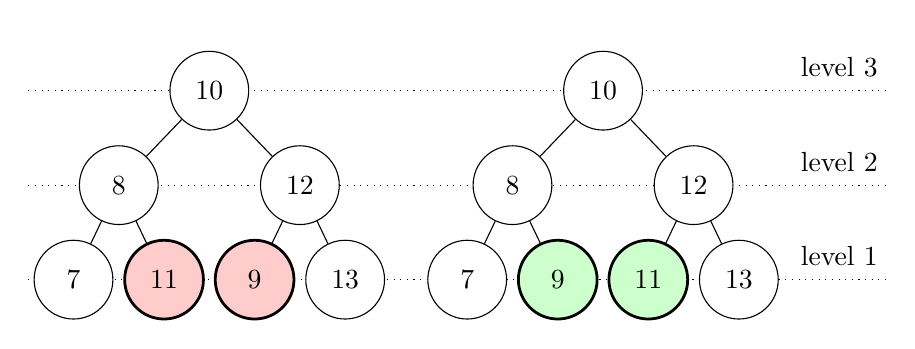
\begin{tikzpicture}
    [ draw
    , every node/.style={minimum size=10mm,fill=white}
    , level/.style={sibling distance = 23mm/#1, level distance=12mm}
    %,    level distance = 1.5cm}
    , sibling distance=8mm
    ]
\draw (-2.3,0) -- (8.6,0)[dotted];
\draw (-2.3,-12mm) -- (8.6,-12mm)[dotted];
\draw (-2.3,-24mm) -- (8.6,-24mm)[dotted];
\node[shape=circle,draw] at (0,0) {10}
    child { node[circle,draw] {8}
        child { node[circle,draw] {7}  }
        child { node[circle,draw,fill=lightred,line width=1pt] {11} }
        }
    child { node[circle,draw] {12}
        child { node[circle,draw,fill=lightred,line width=1pt] {9}  }
        child { node[circle,draw] {13} }
        }
    ;
\node[shape=circle,draw] at (5,0) {10}
    child { node[circle,draw] {8}
        child { node[circle,draw] {7}  }
        child { node[circle,draw,fill=lightgreen,line width=1pt] {9} }
        }
    child { node[circle,draw] {12}
        child { node[circle,draw,fill=lightgreen,line width=1pt] {11}  }
        child { node[circle,draw] {13} }
        }
    ;
\node[fill=none] at (8,3mm) {level 3};
\node[fill=none] at (8,-9mm) {level 2};
\node[fill=none] at (8,-21mm) {level 1};
\end{tikzpicture}
\end{center}

A \textbf{nearest ancestor cover tree} is a simplified cover tree where every point $p$ satisfies the additional invariant that if $q_1$ is an ancestor of $p$ and $q_2$ is a sibling of $q_1$, then
$$
d(p,q_1) \le d(p,q_2)
$$

\end{frame}

%%%%%%%%%%%%%%%%%%%%%%%%%%%%%%%%%%%%%%%%%%%%%%%%%%%%%%%%%%%%%%%%%%%%%%%%%%%%%%%%

\begin{frame}[fragile]{Inserting into a nearest ancestor cover tree}
Inserting into a nearest ancestor cover tree can require rebalancing.
\begin{center}
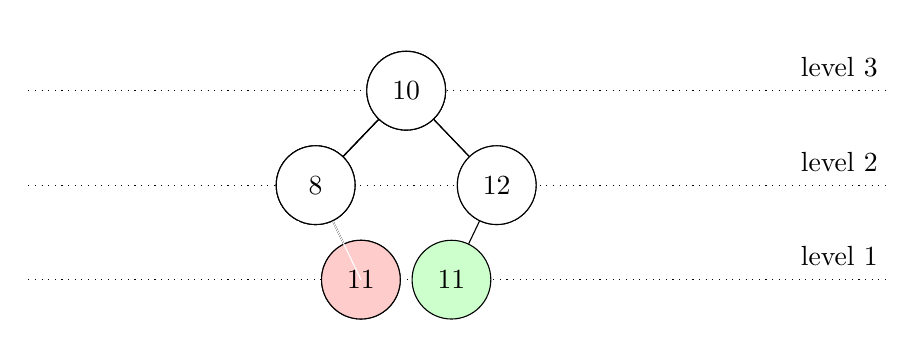
\begin{tikzpicture}
    [ draw
    , every node/.style={minimum size=10mm,fill=white}
    , level/.style={sibling distance = 23mm/#1, level distance=12mm}
    %,    level distance = 1.5cm}
    , sibling distance=8mm
    ]
\draw (-2.3,0) -- (8.6,0)[dotted];
\draw (-2.3,-12mm) -- (8.6,-12mm)[dotted];
\draw (-2.3,-24mm) -- (8.6,-24mm)[dotted];

\uncover<1> {
\node[shape=circle,draw] at (2.5,0) {10}
    child { node[circle,draw] {8}
        child [color=white] {}
        child { node[circle,draw] {11} }
        }
    child [ color=white ] { %node[circle,draw] {12}
        %child { node[circle,draw,fill=lightred,line width=1pt] {9}  }
        %child { node[circle,draw] {13} }
        }
    ;
}

\uncover<2> {
\node[shape=circle,draw] at (2.5,0) {10}
    child { node[circle,draw] {8}
        child [color=white] {}
        child { node[circle,fill=lightred,draw] {11} }
        }
    child  { node[circle,draw] {12}
        %child { node[circle,draw,fill=lightred,line width=1pt] {9}  }
        %child { node[circle,draw] {13} }
        }
    ;
}

\uncover<3> {
\node[shape=circle,draw] at (2.5,0) {10}
    child { node[circle,draw] {8}
        child [color=white] {}
        child [color=white] {}
        }
    child  { node[circle,draw] {12}
        child { node[circle,fill=lightgreen,draw] {11} }
        child [color=white] {}
        %child { node[circle,draw,fill=lightred,line width=1pt] {9}  }
        %child { node[circle,draw] {13} }
        }
    ;
}
\node[fill=none] at (8,3mm) {level 3};
\node[fill=none] at (8,-9mm) {level 2};
\node[fill=none] at (8,-21mm) {level 1};
\end{tikzpicture}
\end{center}

\vspace{0.15in}
No runtime bounds on the rebalancing step.

\vspace{0.15in}
In practice, queries are faster but construction is slower.
\end{frame}

%%%%%%%%%%%%%%%%%%%%%%%%%%%%%%%%%%%%%%%%%%%%%%%%%%%%%%%%%%%%%%%%%%%%%%%%%%%%%%%%

\begin{frame}[fragile]{Comparing cover trees on \emph{construction} time}
\centering
\graphicspath{{slides/paperimg/}}
\input{slides/paperimg/numdist_insert}
\begin{tikzpicture}
    \node[draw,fill=darkred,minimum width=0.03in,minimum height=0.3in] at (0,0) {};
    \node at (0,0.77in) {\small\rotatebox{90}{Original cover tree}};
    \node[draw,fill=darkgreen,minimum width=0.03in,minimum height=0.3in] at (0.15in,0) {};
    \node at (0.15in,0.82in) {\small\rotatebox{90}{Simplified cover tree}};
    \node[draw,fill=blue,minimum width=0.03in,minimum height=0.3in] at (0.3in,0) {};
    \node at (0.3in,1.01in) {\small\rotatebox{90}{Nearest ancestor cover tree}};
    \node[minimum width=0.05in,minimum height=0.5in] at (0.45in,0) {};
    \node at (0.45in,0.6in) {\small\rotatebox{90}{}};
    \node at (0,-0.5in) {};
\end{tikzpicture}
\end{frame}

%%%%%%%%%%%%%%%%%%%%%%%%%%%%%%%%%%%%%%%%%%%%%%%%%%%%%%%%%%%%%%%%%%%%%%%%%%%%%%%%

\begin{frame}[fragile]{Comparing cover trees on \emph{construction and query} time}
\centering
\graphicspath{{slides/paperimg/}}
\input{slides/paperimg/numdist}
\begin{tikzpicture}
    \node[draw,fill=darkred,minimum width=0.03in,minimum height=0.3in] at (0,0) {};
    \node at (0,0.77in) {\small\rotatebox{90}{Original cover tree}};
    \node[draw,fill=darkgreen,minimum width=0.03in,minimum height=0.3in] at (0.15in,0) {};
    \node at (0.15in,0.82in) {\small\rotatebox{90}{Simplified cover tree}};
    \node[draw,fill=blue,minimum width=0.03in,minimum height=0.3in] at (0.3in,0) {};
    \node at (0.3in,1.01in) {\small\rotatebox{90}{Nearest ancestor cover tree}};
    \node[minimum width=0.05in,minimum height=0.5in] at (0.45in,0) {};
    \node at (0.45in,0.6in) {\small\rotatebox{90}{}};
    \node at (0,-0.5in) {};
\end{tikzpicture}
\end{frame}

%%%%%%%%%%%%%%%%%%%%%%%%%%%%%%%%%%%%%%%%%%%%%%%%%%%%%%%%%%%%%%%%%%%%%%%%%%%%%%%%

\begin{frame}[fragile]{All of the cover trees scale similarly}

This experiment uses the protein data and the random walk graph kernel.
\vspace{0.15in}

{
\centering
\graphicspath{{slides/paperimg/}}
\input{slides/paperimg/protein-simple}
\begin{tikzpicture}
    \node[draw,fill=darkred,minimum width=0.03in,minimum height=0.3in] at (0,0) {};
    \node at (0,0.77in) {\small\rotatebox{90}{Original cover tree}};
    \node[draw,fill=darkgreen,minimum width=0.03in,minimum height=0.3in] at (0.15in,0) {};
    \node at (0.15in,0.82in) {\small\rotatebox{90}{Simplified cover tree}};
    \node[draw,fill=blue,minimum width=0.03in,minimum height=0.3in] at (0.3in,0) {};
    \node at (0.3in,1.01in) {\small\rotatebox{90}{Nearest ancestor cover tree}};
    \node[minimum width=0.05in,minimum height=0.5in] at (0.45in,0) {};
    %\node at (0.6in,0.7in) {\small\rotatebox{90}{ dotted lines: construction only}};
    %\node at (0.75in,0.81in) {\small\rotatebox{90}{ solid lines: construction and query}};
    \node at (0,-0.5in) {};
\end{tikzpicture}
}

\end{frame}
